% !TeX root = Thesis.tex
% Điều chỉnh bởi Ta Viet Tai, ICTLAB, FETEL, HCMUS
% Ngày điều chỉnh: 24/03/2024

 %In 1 mặt: oneside
 %In 2 mặt: twoside
\documentclass[a4paper,titlepage,twoside,openright,12pt]{book}
%Kích thước chữ:
\usepackage[fontsize=13pt]{scrextend}

%%===========================================
%%====== Page ref without hyperlink==========
%%=========================================== 
% \usepackage[pageref]{backref}
% \renewcommand\backrefpagesname{}
% \renewcommand\backrefxxx[3]{%
%   {$\textbf{#1}$}%
% }
%%=========================================== 

%%=========================================== 
%%====== Page ref with hyperlink==========
%%=========================================== 
\usepackage[pagebackref]{hyperref}
\hypersetup{
    colorlinks=false,
    linkcolor=red,
    filecolor=magenta,      
    urlcolor=black,
    pdftitle={Thesis},
    pdfauthor={Ta Viet Tai}
    % pdfpagemode=FullScreen,
}
\usepackage{amsmath,amssymb,amsfonts}
\usepackage{cite}
\usepackage{physics}
\usepackage{txfonts}
\usepackage{times}
\usepackage{url}
\usepackage{here}
\usepackage[dvips]{graphicx}
\usepackage{doctorvn,dthook}
\usepackage{color,colortbl}
\usepackage{caption}
\usepackage{subcaption}
\usepackage{rotating}

% Algorithm
\usepackage{algorithm}
\usepackage{algpseudocode}

% Hau usepackage
\usepackage{amsmath}
\usepackage{booktabs}
\usepackage{tabularx}
\usepackage{array}
\usepackage{multirow}
\usepackage{indentfirst}

%Table and figure
\usepackage{svg}
\usepackage{longtable}
\usepackage{pgfplots}
\usetikzlibrary{shapes,arrows,mindmap,decorations.fractals,spy}%

\DeclareUnicodeCharacter{2212}{−}
\usepgfplotslibrary{groupplots,dateplot}
\usetikzlibrary{patterns, shapes.arrows}
\pgfplotsset{compat=newest}
\captionsetup{belowskip=-1.1em}
\pgfplotsset{
  grid style = {
    dash pattern = on 0.05mm off 1mm,
    line cap = round,
    black,
    line width = 0.5pt
  }
}

%%=========================================== 
%========= build fig more faster=============
%%=========================================== 
% \usetikzlibrary{external}
% \tikzexternalize[prefix=fig_tkz/]   
% need using "pdflatex -shell -escape <mainfile>.tex" for the first compiling. Make sure the folder "fig_tkz" is empty. 

%%=====================
%===== Set title=======
%%=====================
% display: on the different line
% hang: on the same line
% \titleformat{\chapter}[hang] 
%   {\Large\bfseries}{\thechapter~~}{0pt}{\Large} %\Large\centering\chaptertitlename~\thechapter

%%=========================================== 
%=========Hyphenation========================
%%=========================================== 

% \hyphenation{op-tical net-works semi-conduc-tor}

%%=========================================== 
%========= Algorithm=========================
%%=========================================== 
% \newcommand{\Input}[1]{\algrenewcommand{\alglinenumber}[1]{Input: \ \setcounter{ALG@line}{\numexpr##1-1}} #1}
% \newcommand{\Step}[1]{\algrenewcommand{\alglinenumber}[1]{Step ##1: } #1}
% \newcommand{\NoNumber}{\algrenewcommand{\alglinenumber}[1]{\setcounter{ALG@line}{\numexpr##1-1} \ \ \ \ \ \ \ \ \ \ }}
% \newcommand{\Output}[1]{\algrenewcommand{\alglinenumber}[1]{Output:\setcounter{ALG@line}{\numexpr##1-1}} #1}


%%=========================================== 
%========= Highlight text====================
%%=========================================== 
\usepackage{color,soul}
\newcommand\highlight[1]{\hl{#1}}
% \renewcommand{\hl}[1]{#1}                 %%  Remove all highlight       
\DeclareRobustCommand{\hlcyan}[1]{{\sethlcolor{cyan!40}\hl{#1}}}
\DeclareRobustCommand{\hlgray}[1]{{\sethlcolor{lightgray}\hl{#1}}}

% Publication
% \usepackage{natbib}
% \usepackage{bibunits}
\usepackage[resetlabels,labeled]{multibib}
\newcites{Pub}{Publication}
% \usepackage[natbib,style=authoryear,refsection=chapter]{biblatex}
% \addbibresource{./0-Bib/Publication.bib}


% Hỗ trợ viết tiếng Việt
\usepackage[T1,T5]{fontenc}
\usepackage[vietnamese]{babel}

% Đánh số cấp 3
\setcounter{secnumdepth}{3}

\begin{document}


\firstuniversity{đại học quốc gia thành phố hồ chí minh}
\seconduniversity{trường đại học khoa học tự nhiên}
\faculty{điện tử -- viễn thông}
\department{Điện tử -- Viễn thông -- Máy tính}
\major{kỹ thuật điện tử}
\departmentId{7520207}
\reporttype{Báo cáo môn học} %luận văn tốt nghiệp | Seminar tốt nghiệp | Báo cáo môn học: Viết báo cáo khoa học bằng LaTeX 

%%============ Name ==================
\title{Kỹ thuật đa người dùng số lượng lớn cho đường lên OFDMA-IDMA dựa trên IEEE 802.11ax} % tên đề tài tiếng việt
\titleEN{Massive Up-Link Multi-User with OFDMA-IDMA
	Combination based on IEEE 802.11ax} % tên đề tài tiếng anh
\author{Tạ Viết Tài} %tên tác giả tiếng việt
\authorEN{Ta Viet Tai} %tên tác giả tiếng anh
\studentid{22C41006}
\supervisor{TS.~Trần~Thị~Thảo~Nguyên~}
\projectname{Các giao thức truyền thông}
% \mail{tttnguyen@hcmus.edu.vn}

%============Tạo trang bìa===============
% \makecoverpage %Report project
\maketitlepage %thesis

\makesubtitlepage	%Tạo trang lót

% \makeassesspage

%========= create foot header =========
% \fancyhf{}
% % \rhead[\rightmark]{\includegraphics[height=1.3cm]{figure/ICTLAB_Logo_withName.pdf}}
% \fancyhead[RO,LE]{\transparent{0.7}\includegraphics[height=1cm]{figure/ICTLAB_Logo.pdf}}
% % \rhead[\rightmark]{\includegraphics[height=1.3cm]{figure/ICTLAB_Logo_withName.pdf}}
% % \cfoot{\thepage}
% \fancyfoot[LE,RO]{\thepage} 
% % \renewcommand{\headrule}{\color[rgb]{0,94,56}}
% \renewcommand{\headrulewidth}{0.4pt}

% Báo cáo tóm tắt:
% \reportSum{
%     \postreportSum
%     \begin{flushleft}
	Tên đề tài: Cải tiến phương pháp đánh giá chất lượng tín hiệu điện tim cho các thiết bị đeo. \\
	Ngành: Kỹ thuật điện tử, hướng Điện tử--Viễn thông và Máy tính. \\
	Mã số ngành: 852020301. \\
	Họ và tên học viên cao học: Tạ Viết Tài. \\
	Khóa đào tạo: 32 (12/2022--12/2024). \\
	Người hướng dẫn khoa học: TS. Trần Thị Thảo Nguyên.\\
	Cơ sở đào tạo: Trường Đại học Khoa học Tự nhiên, ĐHQG.HCM. \\
	\vspace{1.5em}
	\textbf{1. TÓM TẮT NỘI DUNG LUẬN VĂN:}\\
	Content1 \\
	\textbf{2. NHỮNG KẾT QUẢ MỚI CỦA LUẬN VĂN:}\\
	Content2 \\
	\textbf{3. CÁC ỨNG DỤNG/ KHẢ NĂNG ỨNG DỤNG TRONG THỰC TIỄN HAY NHỮNG VẤN ĐỀ CÒN BỎ NGỎ CẦN TIẾP TỤC NGHIÊN CỨU.}\\
	Content3 \\
\end{flushleft}


\vspace{1.5em}
\begin{tblr}{cc}
    \centering
    \textbf{TẬP THỂ CÁN BỘ HƯỚNG DẪN} & \textbf{\hspace{5.0em}HỌC VIÊN CAO HỌC} \\
    \\
    \\
    \\
    TS. Trần Thị Thảo Nguyên & \hspace{5.0em} Tạ Viết Tài
\end{tblr}

\vspace{2.5em}
\begin{center}
    \textbf{XÁC NHẬN CỦA CƠ SỞ ĐÀO TẠO} \\
    \textbf{HIỆU TRƯỞNG}
\end{center}
% }



%Lời cám ơn:
% \acknowledgement{
%     Chúng tôi xin được cảm ơn chương trình Hỗ trợ cho nghiên cứu và giáo dục của 
%     Công ty cổ phần ITR VN đã hỗ trợ kinh phí để nhóm nghiên cứu thực hiện đề tài này. 
%     Đặc biệt, chúng tôi xin chân thành cảm ơn Giám đốc Trần Hoàng Đạt và anh Bùi An Đông của công ty ITR VN 
%     đã tận tình hướng dẫn, hợp tác, cung cấp những kinh nghiệm quý báu, 
%     tạo điều kiện để hỗ trợ nhóm nghiên cứu có những kết quả đầu tiên tốt đẹp.
%     Bên cạnh đó, chúng tôi cũng tỏ lòng biết ơn đến Ban giám hiệu trường Đại học Khoa Học Tự Nhiên, 
%     Ban chủ nhiệm Khoa Điện Tử Viễn Thông, và toàn bộ cán bộ phòng Khoa Học Công Nghệ, 
%     phòng Kế hoạch - Tài chính đã hỗ trợ chúng tôi trong suốt thời gian nghiên cứu.

%     Cuối cùng và cũng là quan trọng nhất, chúng tôi xin được cảm ơn tập thể ICTLAB, 
%     cảm ơn gia đình vì đã luôn luôn âm thầm sát cánh, hỗ trợ chúng tôi trong suốt thời gian vừa qua.
%    %====% 
% \postackEng
% }

\abstractVN{
	Đa truy cập phân chia theo tần số trực giao (OFDMA) được giới thiệu trong chuẩn 802.11ax để giải quyết mối liên quan của các vấn đề truyền dẫn bằng cách chia kênh thành các Đơn vị tài nguyên (RU) được phân bổ cho các Trạm (STA), đặc biệt là trong truyền dẫn đa người dùng Đường lên (UL), nhưng gặp khó khăn với nhiều STA do hạn chế về kích thước RU hoặc băng thông. Đa truy câp phi trực giao (NOMA) là một kỹ thuật mạng không dây được đánh giá cao để khắc phục những vấn đề này. IDMA có thể tận dụng các ưu điểm của NOMA, chẳng hạn như nâng cao hiệu suất phổ, dung lượng STA và tốc độ dữ liệu mà không cần thay đổi kích thước RU hoặc băng thông. Báo cáo này đề xuất sự kết hợp của Đa truy nhập phân chia xen kẽ (IDMA) để tăng số lượng STA trong nhiều người dùng UL vào hệ thống OFDMA 802.11ax hiện có. Việc kết hợp OFDMA và IDMA có thể giảm số lượng STA trên mỗi RU, giảm Nhiễu đa truy cập, đây là vấn đề khi sử dụng IDMA riêng lẻ. Kết quả cho thấy chất lượng Tỷ lệ lỗi bit (BER) giảm đáng kể so với Nhiều đầu vào nhiều người dùng (MU-MIMO), OFDMA và OFDMA-MU-MIMO hiện có trong 802.11ax. Ngoài ra, OFDMA-IDMA hỗ trợ số lượng STA gấp 5 lần OFDMA trong khi vẫn duy trì chất lượng như cũ.

	%======%
	% \postabstractVN %Thời gian và Tên người thực hiện
}

\abstractEng{
	Orthogonal Frequency Division Multiple Access (OFDMA) is introduced in the 802.11 ax standard system to resolve the relevance of transmission problems by splitting the channel into Resource Units (RU) allocated to Stations (STAs), especially in Uplink (UL) multi-user transmission, but struggles with many STAs due to RU size or bandwidth constraints. Non-Othorgonal Multiple Access (NOMA) is a highly appreciated wireless network technique to overcome these issues. The IDMA can take advantage of NOMA, such as enhancing spectrum efficiency, STA capacity, and data rates without RU size or bandwidth changes. This report proposes a combination of Interleave Division Multiple Access (IDMA) to massive the number of STAs in UL multi-user into the existing OFDMA system of 802.11ax. Combining the OFDMA and IDMA can reduce the number of STAs per RU, reducing the Multiple Access Interference, which is the problem when using IDMA individually. The results show a significant decrease in Bit Error Rate (BER) quality compared to existing Multiuser-Multiple Input Multiple Output (MU-MIMO), OFDMA, and OFDMA-MU-MIMO in 802.11ax. In addition, OFDMA-IDMA supports a number of STAs 5 times more than OFDMA while maintaining the same quality.% (BER of approximately. %3\times10^{−4} at SNR = 20 [dB]).

	% \postabstractEng %Thời gian và Tên người thực hiện
}

% Tạo mục lục, danh sách hình vẽ, danh sách bảng
\toc

%%%%%%%%%%%%%%%%%%%%%%%%%%%%%%%%%%%%%%%%%%%%%%%%%%%
%%%%%%%%%%%%%%%%%%%%%%%%%%%%%%%%%%%%%%%%%%%%%%%%%%%
%%%%%%%%%%%%%%%%%%%%%%%%%%%%%%%%%%%%%%%%%%%%%%%%%%%
\makeatletter
\def\cleardoublepage{\clearpage%
	\if@twoside
	\ifodd\c@page\else
	\vspace*{\fill}
	\hfill
	\vspace{-20em}
	\begin{center}
		Trang này được để trống.
	\end{center}
	\vspace{\fill}
	\thispagestyle{empty}
	\newpage
	\if@twocolumn\hbox{}\newpage\fi
	\fi
	\fi
}
\makeatother



\chapter{TỔNG QUAN}
\label{Chap:Intro}
Ngày nay, không thể phủ nhận tỷ lệ các thiết bị điện tử ngày càng tăng lên đáng kể. Theo báo cáo mới nhất của Ericsson Mobility \cite{Ericsson}, vào năm 2023, số lượng đăng ký điện thoại thông minh, PC di động, máy tính bảng và bộ định tuyến di động đã đạt khoảng 7 tỷ thiết bị và được dự đoán sẽ đạt hơn 8,5 tỷ thiết bị vào năm 2030.
Bằng chứng này chứng minh rằng việc sử dụng đồng thời nhiều thiết bị với thông lượng cao và đường truyền đáng tin cậy là một yêu cầu rất lớn trong tương lai. Để đáp ứng những yêu cầu đó trong bối cảnh tài nguyên tần số hạn chế, Ủy ban Tiêu chuẩn LAN/MAN của Hiệp hội Máy tính IEEE đã nỗ lực phát hành các tiêu chuẩn 802.11ax (Wi-Fi 6) \cite{IEEEStd}, tiêu chuẩn này giới thiệu kỹ thuật đa truy cập phân chia theo tần số trực giao \acrshort{OFDMA} để giải quyết mối liên quan của các vấn đề điều khiển truyền dẫn, đặc biệt là trong truyền dẫn đa người dùng \acrshort{MU} đường lên \acrshort{UL}.

 
\acrshort{OFDMA} là một cơ chế quan trọng để sử dụng kênh, chia các kênh có sẵn thành \acrfull{RU} được phân bổ cho \acrshort{STA} riêng lẻ, trong đó mỗi \acrshort{RU} tương ứng với một \acrshort{STA}. OFDMA giảm thiểu một cách hiệu quả các vấn đề về kênh chọn lọc tần số, tập trung vào việc nâng cao chất lượng tín hiệu. Tuy nhiên, tính hiệu quả của nó phải đối mặt với những thách thức trong việc mở rộng quy mô để hỗ trợ nhiều STA, vì việc cung cấp nhiều STA hơn đòi hỏi phải giảm kích thước RU hoặc tăng băng thông.
Để cải thiện số lượng STA mà không thay đổi kích thước hoặc băng thông RU, 802.11ax đã phát hành một tùy chọn kết hợp OFDMA là \acrfull{MU-MIMO}, trong đó mỗi RU sử dụng MU-MIMO. Sử dụng nhiều ăng-ten ở cả phía phát và phía thu sẽ cải thiện hiệu suất phổ và chất lượng truyền mà không cần bổ sung băng thông cũng như tăng công suất nhưng phương pháp này có một số nhược điểm.
Hiệu suất MU-MIMO bị ảnh hưởng mạnh mẽ bởi nhiễu đa truy cập \acrfull{MAI}, khi tăng số lượng STA trong RU, hiệu suất MU-MIMO sẽ giảm đáng kể.
Ngoài ra, việc đánh giá, phân vùng và đồng bộ hóa tín hiệu đòi hỏi các thuật toán xử lý tín hiệu số phức tạp và độ phức tạp triển khai phần cứng cao \cite{MIMO_complex}.

Một bổ sung gần đây cho kho cơ chế Wi-Fi trong tương lai là đa truy cập phi trực giao \acrshort{NOMA}, cho phép truyền đồng thời nhiều tín hiệu trong cùng một tài nguyên tần số thời gian. Mặc dù NOMA không được tích hợp vào tiêu chuẩn 802.11ax nhưng nhiều nghiên cứu khác nhau cho thấy khả năng tương thích ngược của nó với các tiêu chuẩn IEEE 802.11 hiện có. Đáng chú ý, Evgeny Khorov và các cộng sự đã trình bày nguyên mẫu thiết bị Wi-Fi đầu tiên hỗ trợ NOMA \cite{NOMA_WiFi}. Công trình của họ đã chứng minh việc giảm tỷ lệ lỗi bit \acrshort{BER} bằng cách kết hợp NOMA với Wi-Fi, như được nêu bật trong \cite{PhaseNoise}.
Nhiều nghiên cứu của NOMA tập trung vào miền công suất, cung cấp cho STA các hệ số công suất khác nhau và sử dụng \acrfull{SIC} để phát hiện tín hiệu. Tuy nhiên, NoMA miền quyền lực gặp phải thách thức về khả năng mở rộng, vì việc đáp ứng các điều kiện \acrshort{SIC} cho nhiều STA trở nên phức tạp. 
Ngoài ra, tính chất tuần tự của SIC, tiến triển từ STA yếu đến mạnh, có thể dẫn đến thời gian xử lý tăng lên, có khả năng vi phạm yêu cầu \acrfull{SIFS} trong hệ thống 802.11. Để giải quyết những hạn chế này, bài viết này sử dụng NOMA trong miền mã \acrfull{IDMA}. IDMA, một biến thể \acrfull{CDMA}, sử dụng mã xen kẽ để phân biệt các STA, dẫn đến bộ thu có độ phức tạp thấp có khả năng phát hiện tín hiệu song song \cite{IDMA}. Ngược lại với Đa truy cập phân chia theo tần số trực giao (OFDMA), IDMA cho phép tất cả STA sử dụng đồng thời tất cả các sóng mang con, loại bỏ chi phí dư thừa, độ phức tạp tính toán và các mối lo ngại về độ trễ \cite{IDMA_Per}.

Bài viết này đề xuất sự kết hợp các hệ thống OFDMA-IDMA dựa trên kiến trúc 802.11ax.
Sự kết hợp này có thể tăng đáng kể số lượng STA mà không làm giảm kích thước RU hoặc tăng băng thông như OFDMA, do đó cải thiện hiệu quả băng thông.
Ngoài ra, OFDMA-IDMA còn cho phép có nhiều STA hơn mà không cần nhiều mã xen kẽ như IDMA truyền thống. Bằng cách sử dụng lại các mã xen kẽ ở các RU khác nhau, có thể tăng tính ngẫu nhiên của mã được sử dụng trong một RU, nhờ đó tăng hiệu quả giải mã ở máy thu.
Hơn nữa, bằng cách chia số lượng STA thành RU, kỹ thuật OFDMA-IDMA có thể làm giảm ảnh hưởng của nhiễu liên ký tự \acrfull{ISI} và đặc biệt là \acrshort{MAI}.
Hơn nữa, hệ thống được đề xuất tăng số lượng STA được truyền đồng thời trên đường lên và giảm BER so với OFDMA-MU-MIMO. Bài viết này cũng sử dụng phương pháp điều chế bậc cao đơn giản hóa \cite{IDMAHighOder} từ nghiên cứu trước đây của chúng tôi, giúp việc giải mã IDMA đơn giản hơn MU-MIMO.
Ngoài ra, bài viết này sử dụng Kết hợp tỷ lệ tối đa \acrshort{MRC} tại AP để đảm bảo chất lượng tín hiệu và sử dụng kênh \acrshort{MIMO} pha đinh đa đường mô hình B TGax \cite{TGax} để đảm bảo độ bền và tính thực tế. Kết quả mô phỏng dựa trên hệ thống 802.11ax cho thấy hiệu suất BER được cải thiện so với các kỹ thuật hiện có như MU-MIMO, OFDMA và OFDMA-MU-MIMO.

Cấu trúc của bài báo cáo bao gồm 5 chương như Hình \ref{fig:Struc}:

\textbf{Chương \ref{Chap:Intro}}: Giới thiệu tổng quan về các kỹ thuật đa truy cập đường lên hiện có trong 802.11ax. Các ưu khuyết điểm và lý do đề xuất kỹ thuật OFDMA-IDMA.

\textbf{Chương \ref{Chap:II}}: Giới thiệu cơ sở lý thuyết của IDMA và cấu trúc bộ thu IDMA với nhiều ăng-ten. 

\textbf{Chương \ref{Chap:III}}: Đề xuất kiến trúc mô hình bộ phát và thu OFDMA-IDMA dựa trên chuẩn 802.11ax. 

\textbf{Chương \ref{Chap:IV}}: So sánh tỉ lệ lỗi của hệ thống OFDMA-IDMA với các kỹ thuật đa truy cập hiện có của chuẩn 802.11ax. 

\textbf{Chương \ref{Chap:V}}: Bàn luận ưu và nhược điểm của OFDMA-IDMA và hướng phát triễn. 

\begin{figure}[H]
    \centering
    \begin{tikzpicture}[node distance = 2cm, auto]
    \tikzstyle{block} = [rectangle, draw, text width=0.8\linewidth, 
    text centered, rounded corners, minimum height=2.3em]
    \tikzstyle{line} = [draw, -latex', line width = 0.1em]
    % Place nodes
    \node [block] (C1) {\textbf{Chương \ref{Chap:Intro}}: Tổng quan};
    \node [block, below of=C1] (C2) {\textbf{Chương \ref{Chap:II}}: Tổng quan hệ thống IDMA};
    \node [block, below of=C2] (C3) {\textbf{Chương \ref{Chap:III}}: Đề xuất OFDMA-IDMA dựa trên chuẩn 802.11ax};
    \node [block, below of=C3] (C4) {\textbf{Chương \ref{Chap:IV}}: Kết quả mô phỏng hiệu năng};
    \node [block, below of=C4] (C5) {\textbf{Chương \ref{Chap:V}}: Kết luận và hướng phát triển};
    % Draw edges
    \path [line] (C1) -- (C2);
    \path [line] (C2) -- (C3);
    \path [line] (C3) -- (C4);
    \path [line] (C4) -- (C5);

\end{tikzpicture}
    \caption{Cấu trúc báo cáo.}
    \label{fig:Struc}
\end{figure}


\chapter{TỔNG QUAN HỆ THỐNG IDMA}
\label{Chap:II}
\section{Kiến trúc bộ phát}\label{IIA}

Quá trình thực hiện mã hóa và giả mã IDMA của $N$ STAs được diễn tả ở Hình \ref{fig:IDMASystem}, trong đó khối trãi tín hiệu và đan xen là hai quá trình quan trọng khi thực hiện IDMA \cite{IDMA_LiPing}. Dữ liệu $d_n$ của mỗi STA được trãi ra bởi chuỗi chip $c$ = [-1 1 $\dots$ -1 1], với \acrshort{SF} là hệ số trãi với giá trị bằng chiều dài của chuỗi chip. Điều kiện tiên quyết để IDMA hoạt động là mỗi STA thứ $n$ sẽ được trộn bởi một mã đan xen riêng biệt $\pi_n$, giả sử chuỗi $\pi_n$ là ngẫu nhiên độc lập với nhau.

\section{Kiến trúc bộ thu}\label{IIB}

Tín hiệu nhận được ở phía thu có thể được công thức hóa bởi \eqref{eq:1}, với tín hiệu phát và thu tương ứng với $[\mathbf{x}_1 \cdots \mathbf{x}_N]^\top$ và $[\mathbf{y}_1 \cdots \mathbf{y}_K]^\top$. $\mathbf{x}_n$ là vector tín hiệu của STA thứ $n$, $\mathbf{y}_k$ là vector tín hiệu nhận tại ăng-ten thứ $k$ của AP và nhiễu phía thu tại ăng-ten theo phân phối Gauss phức với $\mathbf{N} \sim \mathcal{N}_\mathbb{C}(\mathbf{0},\sigma^2\mathbf{I}_K)$

\begin{equation}
	\begin{bmatrix}
		\mathbf{y}_1 \\
		\vdots       \\
		\mathbf{y}_K \\
	\end{bmatrix}
	=
	\begin{bmatrix}
		\mathbf{h}_{1,1} & \cdots & \mathbf{h}_{1,N} \\
		\vdots           & \ddots & \vdots           \\
		\mathbf{h}_{K,1} & \cdots & \mathbf{h}_{K,N}
	\end{bmatrix}
	\times
	\begin{bmatrix}
		\mathbf{x}_1 \\
		\vdots       \\
		\mathbf{x}_N \\
	\end{bmatrix}
	+
	\mathbf{N}.
	\label{eq:1}
\end{equation}

Thành phần chính yếu trong bộ giải mã IDMA chính là \acrfull{ESE} được dùng để tính toán tỉ số \acrfull{LLR} cho vector tín hiệu $\mathbf{x}_n $ = $[x_n(1),\dots,x_n(j),\dots,x_n(J)]$ của STA thứ $n$ STA và bộ giải mã dựa trên xác xuất hậu nghiệm \acrfull{APP}.

\subsection{Elementary Signal Estimator} \label{sub2.1}

Vector tín hiệu tại ăng-ten thứ $k$ có thể được viết lại như \eqref{eq:2}

\begin{figure}
	\centering
	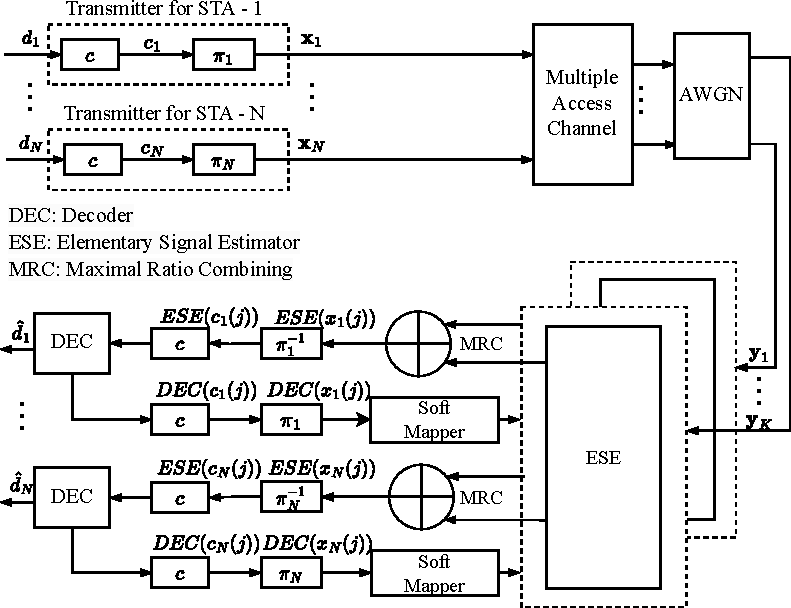
\includegraphics[width = 0.75\linewidth]{figure/Chap2/IDMA_Tx_Rx_structure-2_k2opt.pdf}
	\caption{Hệ thống IDMA với đa ăng-ten nhận.}
	\vspace{-1em}
	\label{fig:IDMASystem}
\end{figure}

\begin{equation}
	\mathbf{y}_k = \mathbf{h}_{k,n} \times \mathbf{x}_n
	+ \overbrace{\sum_{n' \neq n}\mathbf{h}_{k,n'} \times \mathbf{x}_{n'}
		+ \mathbf{N}}^{\zeta_{k,n}},
	\label{eq:2}
\end{equation}%\vspace{-0.5em}
trong đó $\zeta_{k,n}$ là thành phần nhiễu cộng can nhiễu tại ăng-ten $k$. Từ định lý giới hạn trung tâm, ta có thể xấp xỉ $\zeta_{k,n}$ như một biến ngẫu nhiên có phần bố Gaus, và tín hiệu $\mathbf{y}_k$ có thể ghi như hàm PDF như \eqref{eq:3}
\begin{equation}
	% \begin{split}
	p(y_k(j)\mid x_n(j)=\pm 1) =
	\frac{1}{\sqrt{2\pi}\text{Var}(\zeta_{k,n}(j))}
	e^{\mathord{-}\dfrac{(y_k(j)\mathord{-}(\pm h_{k,n}(j)\mathord{+}\mathbb{E}(\zeta_{k,n}(j))))^2}{2\text{Var}(\zeta_{k,n}(j))}},
	% \end{split}
	\label{eq:3}
\end{equation}
trong đó $\mathbb{E}\{\cdot\}$ và Var$\{\cdot\}$ tương ứng là giá trị ky vọng và phương sai của phân bố. Định lý giới hạn trung tâm đúng khi áp dụng cho một lượng lớn phân bố ngẫu nhiên độc lập với nhau, và nó thích hợp để dùng trong IDMA. Thuật toán \ref{alg:ESE} với đầu vào là $\mathbf{y}_k$ và $\mathbf{h}_{k,n}$ được dùng để tính toán tỉ số LLR $x_{k,n}(j)$, với $\{\cdot\}^*$ và $\{\cdot\}^\top$ lần lượt là phép chuyển vị phức và phép chuyển vị.

Thuật toán \ref{alg:ESE} tính toán giá trị ESE cho STA thứ $n$ tại ăng-ten $k$ và các giá trị này sẽ được tính lại sau mỗi lần lặp, phần cập nhập sẽ được nói rõ ở phần \ref{update}.
Giá trị bit $b_{I,\nu}$ được quyết định cứng là $\beta$ (tương tự cho $b_{Q,\nu}$) được cho bởi
\begin{equation}
	p(b_{I,\nu} = \beta \mid y_{k,n}(j)) > p(b_{I,\nu} = (1-\beta) \mid y_{k,n}(j)). \label{eq:4}
\end{equation}

\begin{algorithm}
	% \vspace{-0.5em}
	\caption{ESE Detection Algorithm.}\label{alg:ESE}
	% \footnotesize
	\begin{algorithmic}[1]
		\Procedure{ESE}{$\mathbf{y}_k,\mathbf{h}_{k,n}$}

		% \While{$j \leq J$}               
		\State $\mathbb{E}(x_{k,n}(j)) = 0$     \Comment{Khởi tạo ban đầu}

		\State $\mathbb{E}(y_{k,n}(j)) = 0$

		\State $\textbf{Cov}(x_{k,n}(j)) = \textbf{I}_2$
		\State $\textbf{Cov}(y_{k,n}(j)) = \sigma^2\textbf{I}_2$

		\State $\textbf{R}_{k,n}(j)=
			\begin{bmatrix}
				\Re(h_{k,n}(j)) & -\Im(h_{k,n}(j)) \\
				\Im(h_{k,n}(j)) & \Re(h_{k,n}(j))
			\end{bmatrix}$

		\State $\textbf{Cov}(\zeta_{k,n}(j))=\textbf{Cov}(y_{k,n}(j))~-~\textbf{R}_{k,n}(j)\textbf{Cov}(x_{k,n}(j)) \textbf{R}_{k,n}(j)^\top$

		\State $\text{Var}(\tilde{\zeta}_{k,n}(j)) = \textbf{R}_{k,n}(j)^\top \textbf{Cov}(\zeta_{k,n}(j)) \textbf{R}_{k,n}(j)$

		\State $\mathbb{E}(\tilde{\zeta}_{k,n}(j)) = h_{k,n}^{*}(j)(\mathbb{E}(y_{k,n}(j)) - h_{k,n}(j) \mathbb{E}(x_{k,n}(j)))$

		\State $ESE(x_{k,n}(j))~=~\dfrac{2\lvert h_{k,n}\rvert^2\overbrace{(h_{k,n}^{*}(j) y_{k,n}(j) - \mathbb{E}(\tilde{\zeta}_{k,n}(j)))}^{LLR}}{\text{Var}(\tilde{\zeta}_{k,n}(j))}$                                  \Comment{Tính toán ESE}

		% \EndWhile  

		\EndProcedure
	\end{algorithmic}
\end{algorithm}

Tỉ số LLR được tính bởi
\begin{equation}
	% \begin{split}
	LLR(b_{I,\nu})  \triangleq \log \left(\dfrac{p(b_{I,\nu} \mathord{=} 1 \mid y_{k,n}(j))}{p(b_{I,\nu} \mathord{=} 0 \mid y_{k,n}(j))}\right)
	\mathord{=} \log \left(\dfrac{\sum_{\alpha\in S_{I,\nu}^{(1)}}p(x_{k,n}(j)\mathord{=} \alpha\mid y_{k,n}(j))}{\sum_{\alpha\in S_{I,\nu}^{(0)}}p(x_{k,n}(j)\mathord{=} \alpha\mid y_{k,n}(j))}\right),
	% \end{split}
	\label{eq:5}
\end{equation}
sử dụng lý thuyết Baye và giả sử các symbol có phân phối như nhau, \eqref{eq:5} được viết lại
\begin{equation}
	LLR(b_{I,\nu})\mathord{=}\log \left(\dfrac{\sum_{\alpha\in S_{I,\nu}^{(1)}}p(y_{k,n}(j) \mid x_{k,n}(j)\mathord{=} \alpha)}
		{\sum_{\alpha\in S_{I,\nu}^{(0)}}p(y_{k,n}(j) \mid x_{k,n}(j)\mathord{=} \alpha)}\right).
	\label{eq:6}
\end{equation}

một bài toán tối ưu để tính tỉ số LLR một cách đơn giản hơn khi dùng khai triển Taylor cho biểu thức $\log (1+z)$ khi $z \ll 1$, dễ dàng thấy được: $\log \Sigma_jz_j \approx \text{max}_j \log z_j$, khi đó \eqref{eq:6} được viết gần đúng bởi \eqref{eq:7}
\begin{equation}
	LLR(b_{I,\nu}) \mathord{\approx}\log \left(\dfrac{\max_{\alpha\in S_{I,\nu}^{(1)}} p(y_{k,n}(j) \mathord{\mid} x_{k,n}(j)\mathord{=} \alpha)}
		{\max_{\alpha\in S_{I,\nu}^{(0)}} p(y_{k,n}(j) \mathord{\mid} x_{k,n}(j)\mathord{=} \alpha)}\right),
	\label{eq:7}
\end{equation}
với $\alpha$ là một điểm trên chòm sao. Hình \ref{fig:16-QAM} cho thấy vùng quyết định $S_{I,\nu}^{(s)}$ cho thành phần thực $b_{I,\nu}$ và $S_{Q,\nu}^{(s)}$ cho thành phần ảo $b_{Q,\nu}$ với $s=[0,1]$ trong trường hợp 16-QAM. Dễ dàng nhận thấy chúng được phân định bởi ranh giới ngang hoặc dọc. Do đó, hai ký hiệu trong hai tập con gần tín hiệu cân bằng nhận được nhất luôn nằm trên cùng một hàng nếu ranh giới phân vùng là dọc (bit $b_{I,1}$ và $b_{I,2}$ trong Hình \ref{fig:16-QAM}) hoặc trong cùng một cột nếu ranh giới nằm ngang (bit $b_{Q,1}$ và $b_{Q,2}$ trong Hình \ref{fig:16-QAM}). Kết quả là, khi sử dụng \eqref{eq:3} trong \eqref{eq:7}, các giá trị bit mềm cuối cùng có thể được biểu thị bằng khoảng cách Euclide tối thiểu như sau
\begin{equation}
	\begin{split}
		LLR(b_{I,\nu}) =&\dfrac{\absolutevalue{h_{k,n}(j)}^2}{4} \Bigg\{ \min_{\alpha_I \in S_{I,\nu}^{'(0)}}(\Re(y_{k,n}(j)) - \alpha_I)^2 - \min_{\alpha_I \in S_{I,\nu}^{'(1)}}(\Re(y_{k,n}(j)) - \alpha_I)^2 \Bigg\}\\
		\triangleq & \absolutevalue{h_{k,n}(j)}^2 \times D_{I,\nu},
	\end{split}
	\label{eq:8}
\end{equation}
trong đó $S_{I,\nu}^{'(s)} \triangleq \Re(S_{I,\nu}^{(s)})$.

\begin{figure}
	\centering
	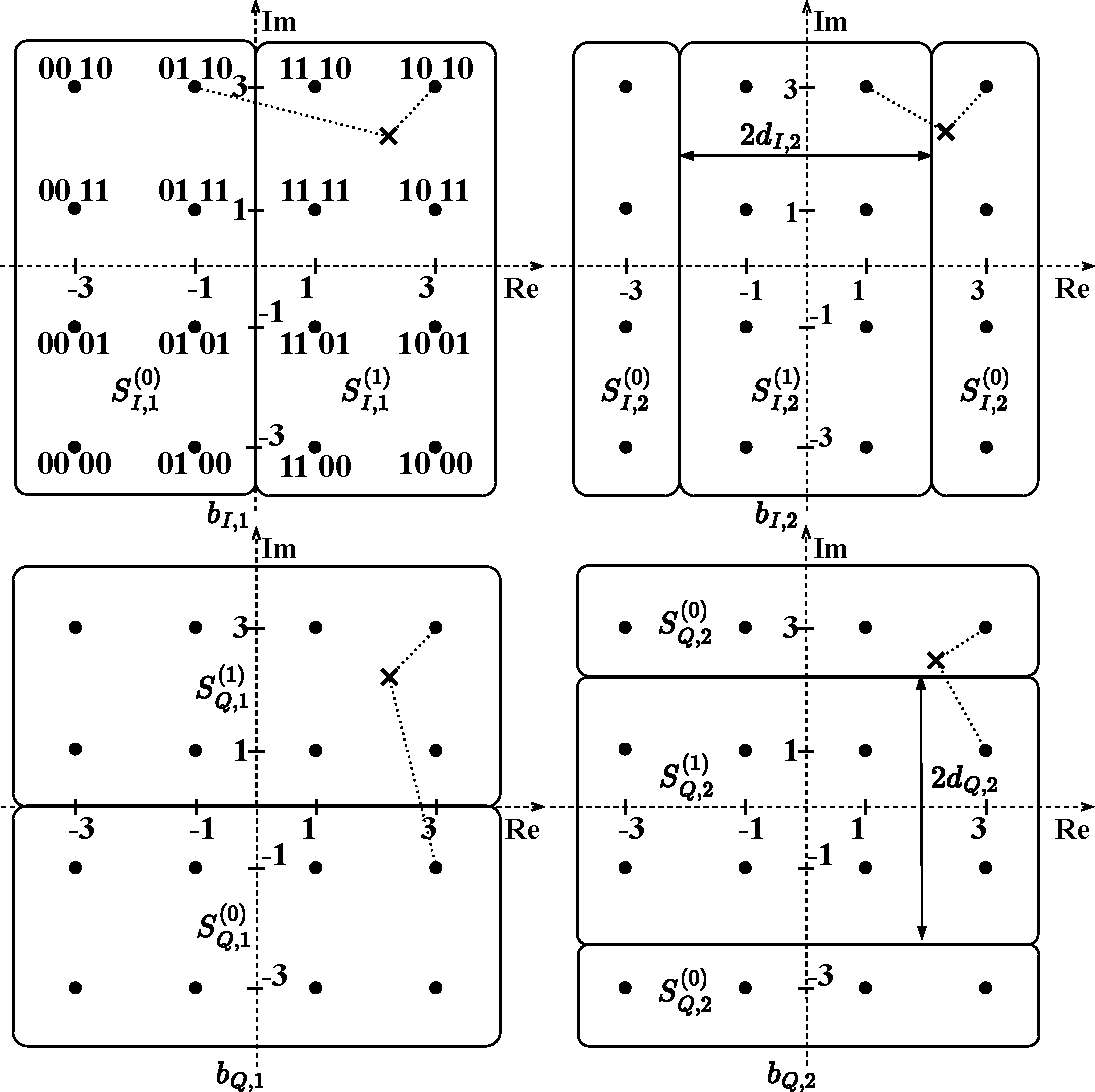
\includegraphics[width=0.75\linewidth]{figure/Chap2/16-QAM.pdf}
	\caption{Giải điểu biến 16-QAM đơn giản.}
	\label{fig:16-QAM}
	\vspace{-1em}
\end{figure}

Việc tính toán chính xác $D_{I,\nu}$, $D_{Q,\nu}$ trong \eqref{eq:8} yêu cầu nhiều phép tính của hàm logarit và việc thực hiện phức tạp hơn. Bài viết này triển khai \cite{SimpleDemap} để tính giá trị LLR gần đúng. Các giá trị $D_{I,\nu}$ và $D_{Q,\nu}$ cho 16-QAM được tính bởi
\begin{equation}
	D_{I,1}=\left\{
	\begin{matrix}
		2\Re(y_{I,k,n}(j))+2 & \Re(y_{k,n}(j)) < -2,          \\
		\Re(y_{I,k,n}(j))    & -2\leq \Re(y_{k,n}(j)) \leq 2, \\
		2\Re(y_{I,k,n}(j))-2 & \Re(y_{k,n}(j)) > 2,
	\end{matrix}
	\right. \label{eq:9}
\end{equation}
\begin{equation}
	\begin{matrix}
		D_{I,2}=-\absolutevalue{\Re(y_{I,k,n})} & \text{for all } \Re(y_{I,k,n}).
	\end{matrix}
	\label{eq:10}
\end{equation}

Thay thế phần $LLR$ ở dòng 10 trong thuật toán \ref{alg:ESE} bằng \eqref{eq:8}, công thức $ESE$ có thể được biểu diễn dưới dạng
\begin{equation}
	ESE(\Re(x_{k,n}(j)))~=~\dfrac{2\lvert h_{k,n}\rvert^4D_{I,\nu}}
	{\text{Var}(\tilde{\zeta}_{k,n}(j))},
\end{equation}
và $ESE(\Im(x_{k,and}(j)))$ được tính theo cách tương tự.


\subsection{Khối DEC}

Sau khi tính toán giá trị LLR, báo cáo này sử dụng kỹ thuật \acrshort{MRC} để đat tỷ số tín hiệu trên nhiễu \acrshort{SNR} cao nhất có thể đạt được tại AP. Sau đó, quá trình loại bỏ xen kẽ sẽ được thực hiện với cùng mã bộ xen $\pi_n$, được sử dụng cho STA thứ $n$ tại máy phát. Tiếp theo, giá trị chip LLR được so sánh với ngưỡng. Nếu các giá trị này lớn hơn ngưỡng, chúng sẽ bị cắt bớt thành giá trị ngưỡng.

\subsection{Cập nhật giá trị trung bình và phương sai} \label{update}
Sau khi tính toán DEC, IDMA cần cập nhật giá trị trung bình và phương sai cho lần lặp tiếp theo. Phần cập nhật bao gồm bộ trãi mã, bộ xen kẽ và bộ ánh xạ mềm. Đầu ra của quá trình khử trải phổ là các LLR bên ngoài cho $y_{k,n}(j)$ Sau đó, các LLR này được sử dụng để tạo số liệu thống kê trong \eqref{eq:12}, \eqref{eq:13}
\begin{subequations}
	\begin{equation}
		\mathbb{E}(x_{k,n}(j)) = \sum_{\nu = 0}^{2^{N_{bpsc}}-1} (p \mathord{+}iq)_\nu \mathord{\times} \left(\dfrac{e^{DEC(\hat{a}_n(j))}}{1 \mathord{+} e^{DEC(\hat{a}_n(j))}}\right)_\nu,
		\label{eq:12}
	\end{equation}
	\begin{equation}
		\begin{split}
			\textbf{Cov}(x_{k,n}(j))\mathord{=}
			& \diag\big(\Re(\text{Var}(x_{k,n}(j))) \mathord{-} \Re(\mathbb{E}(x_{k,n}(j)))^2, \\
			& \Im(\text{Var}(x_{k,n}(j))) \mathord{-} \Im(\mathbb{E}(x_{k,n}(j)))^2\big),
		\end{split}
		\label{eq:13}
	\end{equation}
\end{subequations}
trong đó $N_{bpsc}$ là số bit trên mỗi ký hiệu, $p$ và $q$ là các giá trị được lấy bởi trục $\Re$ và $\Im$ (ví dụ: các giá trị là $\{$-3, -1, +1, +3$\}$ cho 16-QAM).


\chapter{ĐỀ XUẤT OFDMA-IDMA DỰA TRÊN CHUẨN 802.11AX}
\label{Chap:III}
\section{Mô hình phía phát}

Hình \ref{fig:Transmitter} biểu diễn OFDMA-MU-MIMO trong tiêu chuẩn 802.11ax và hệ thống OFDMA-IDMA được đề xuất. Có thể thấy rằng mô hình đề xuất trong Hình \ref{fig:Proposed_OFDMA-IDMA} có khối tương tự như OFDMA-MU-MIMO trong Hình \ref{fig:Old-OFDMA-MU-MIMO}. Tuy nhiên, trong mô hình đề xuất, thay vì thực hiện quá trình phân luồng không gian, các STA chỉ thực hiện quá trình trải và xen kẽ.
Trong báo cáo này, mã xen kẽ được sử dụng hiệu quả hơn IDMA thông thường bằng cách kết hợp với OFDMA; các mã này được sử dụng lại trong các RU khác nhau, nhằm tăng số lượng STA trong khi vẫn không làm tăng số lượng mã bộ chèn.
Ngoài ra, để tương thích với LDPC trong chuẩn 802.11ax khi thêm khối bộ mã hóa IDMA vào quy trình, các tham số $N_{pld,u}$ và $N_{avbits,u}$ trong phương trình (27-29) và phương trình(27-80) trong \cite{IEEEStd} được thay thế bằng \eqref{eq:14} và \eqref{eq:15}
% \vspace{-0.5em}
\begin{equation}
	\begin{split}
		N_{pld,u} = &{\text{SF}}^{-1}((N_{\text{SYM,init}}-m_{\text{STBC}} \mathord{\times} \text{SF}) \mathord{\times} N_{\text{DBPS},u} \\
		&+ m_{\text{STBC}} \mathord{\times} N_{\text{DBPS,last,init},u}),
	\end{split}
	\label{eq:14}
\end{equation}

\begin{equation}
	\begin{split}
		N_{avbits,u} = &{\text{SF}}^{-1}((N_{\text{SYM,init}}-m_{\text{STBC}} \mathord{\times} \text{SF}) \mathord{\times} N_{\text{CBPS},u} \\
		&+ m_{\text{STBC}} \mathord{\times} N_{\text{CBPS,last,init},u}),
	\end{split}
	\label{eq:15}
\end{equation}
với $N_{\text{DBPS,last,init},u}$, $N_\text{SYM,init}$, $m_{\text{STBC}}$, $N_{\text{DBPS}, u}$, $N_{\text{CBPS},u}$, $N_{\text{CBPS,last,init},u}$ có cùng định nghĩa trong \cite{IEEEStd} và SF là hệ số trải phổ sử dụng trong IDMA.
\begin{figure}
	\centering
	\begin{subfigure}{0.49\linewidth}
		\centering
		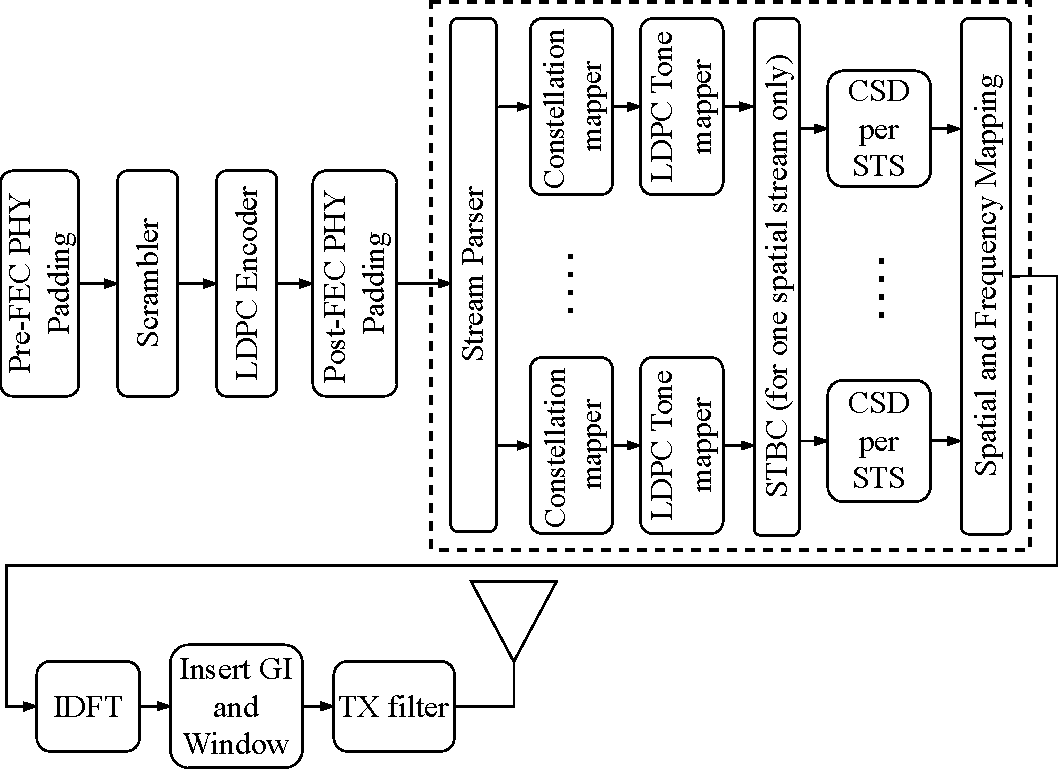
\includegraphics[width=1.2\linewidth, angle = -90]{figure/chap3/MU-MIMOTx_k2opt.pdf}
		\caption{OFDMA-MU-MIMO 802.11ax.}
		\label{fig:Old-OFDMA-MU-MIMO}
	\end{subfigure}
	\vspace{1em}
	%==============
	\begin{subfigure}{0.49\linewidth}
		\centering
		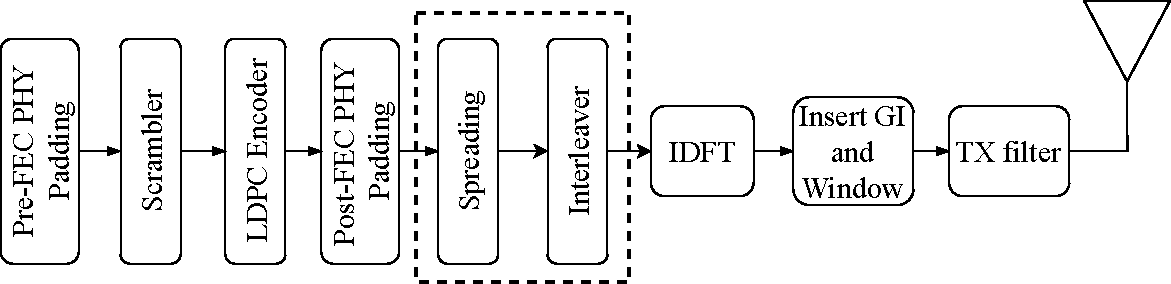
\includegraphics[width=\linewidth, angle = -90]{figure/chap3/IDMA_Tx_Rx_structure-Trang-4_k2opt.pdf}
		\caption{OFDMA-IDMA đề xuất dựa trên 802.11ax.}
		\label{fig:Proposed_OFDMA-IDMA}
	\end{subfigure}

	\caption{Kiến trúc đường lên với mã hóa LDPC.}
	% \vspace{-1em}
	\label{fig:Transmitter}
\end{figure}
\section{Mô hình phía thu}

Để xác thực tính khả thi của hệ thống được đề xuất trong môi trường WLAN, chúng tôi trình bày cách triển khai bộ thu được mô tả trong Hình \ref{fig:OFDMA-IDMARx}. Kiến trúc bộ thu phản chiếu bộ thu 802.11 tiêu chuẩn cho đến giai đoạn ESE, nơi quá trình xử lý IDMA bắt đầu. Bài viết này sử dụng giải mã IDMA kết hợp với MRC như trong Hình \ref{fig:IDMASystem}. Việc lựa chọn số lần lặp trong giải mã IDMA là rất quan trọng, ảnh hưởng đến cả hiệu suất và độ trễ. Sau mỗi lần lặp, các giá trị thống kê về nhiễu và nhiễu được cập nhật cho các phép tính tiếp theo, cải thiện độ chính xác với số lần lặp tăng lên. Tuy nhiên, số lần lặp nhiều hơn cũng có nghĩa là độ trễ tính toán cao hơn. Để đáp ứng mục tiêu độ trễ 10 $\mu s$ phù hợp với tiêu chuẩn 802.11, chúng tôi áp dụng bốn lần lặp, như được xác định trong \cite{UL-OFDM-IDMA} với SF là 2 trong thiết lập của chúng tôi.

\begin{figure}[H]
	\centering
	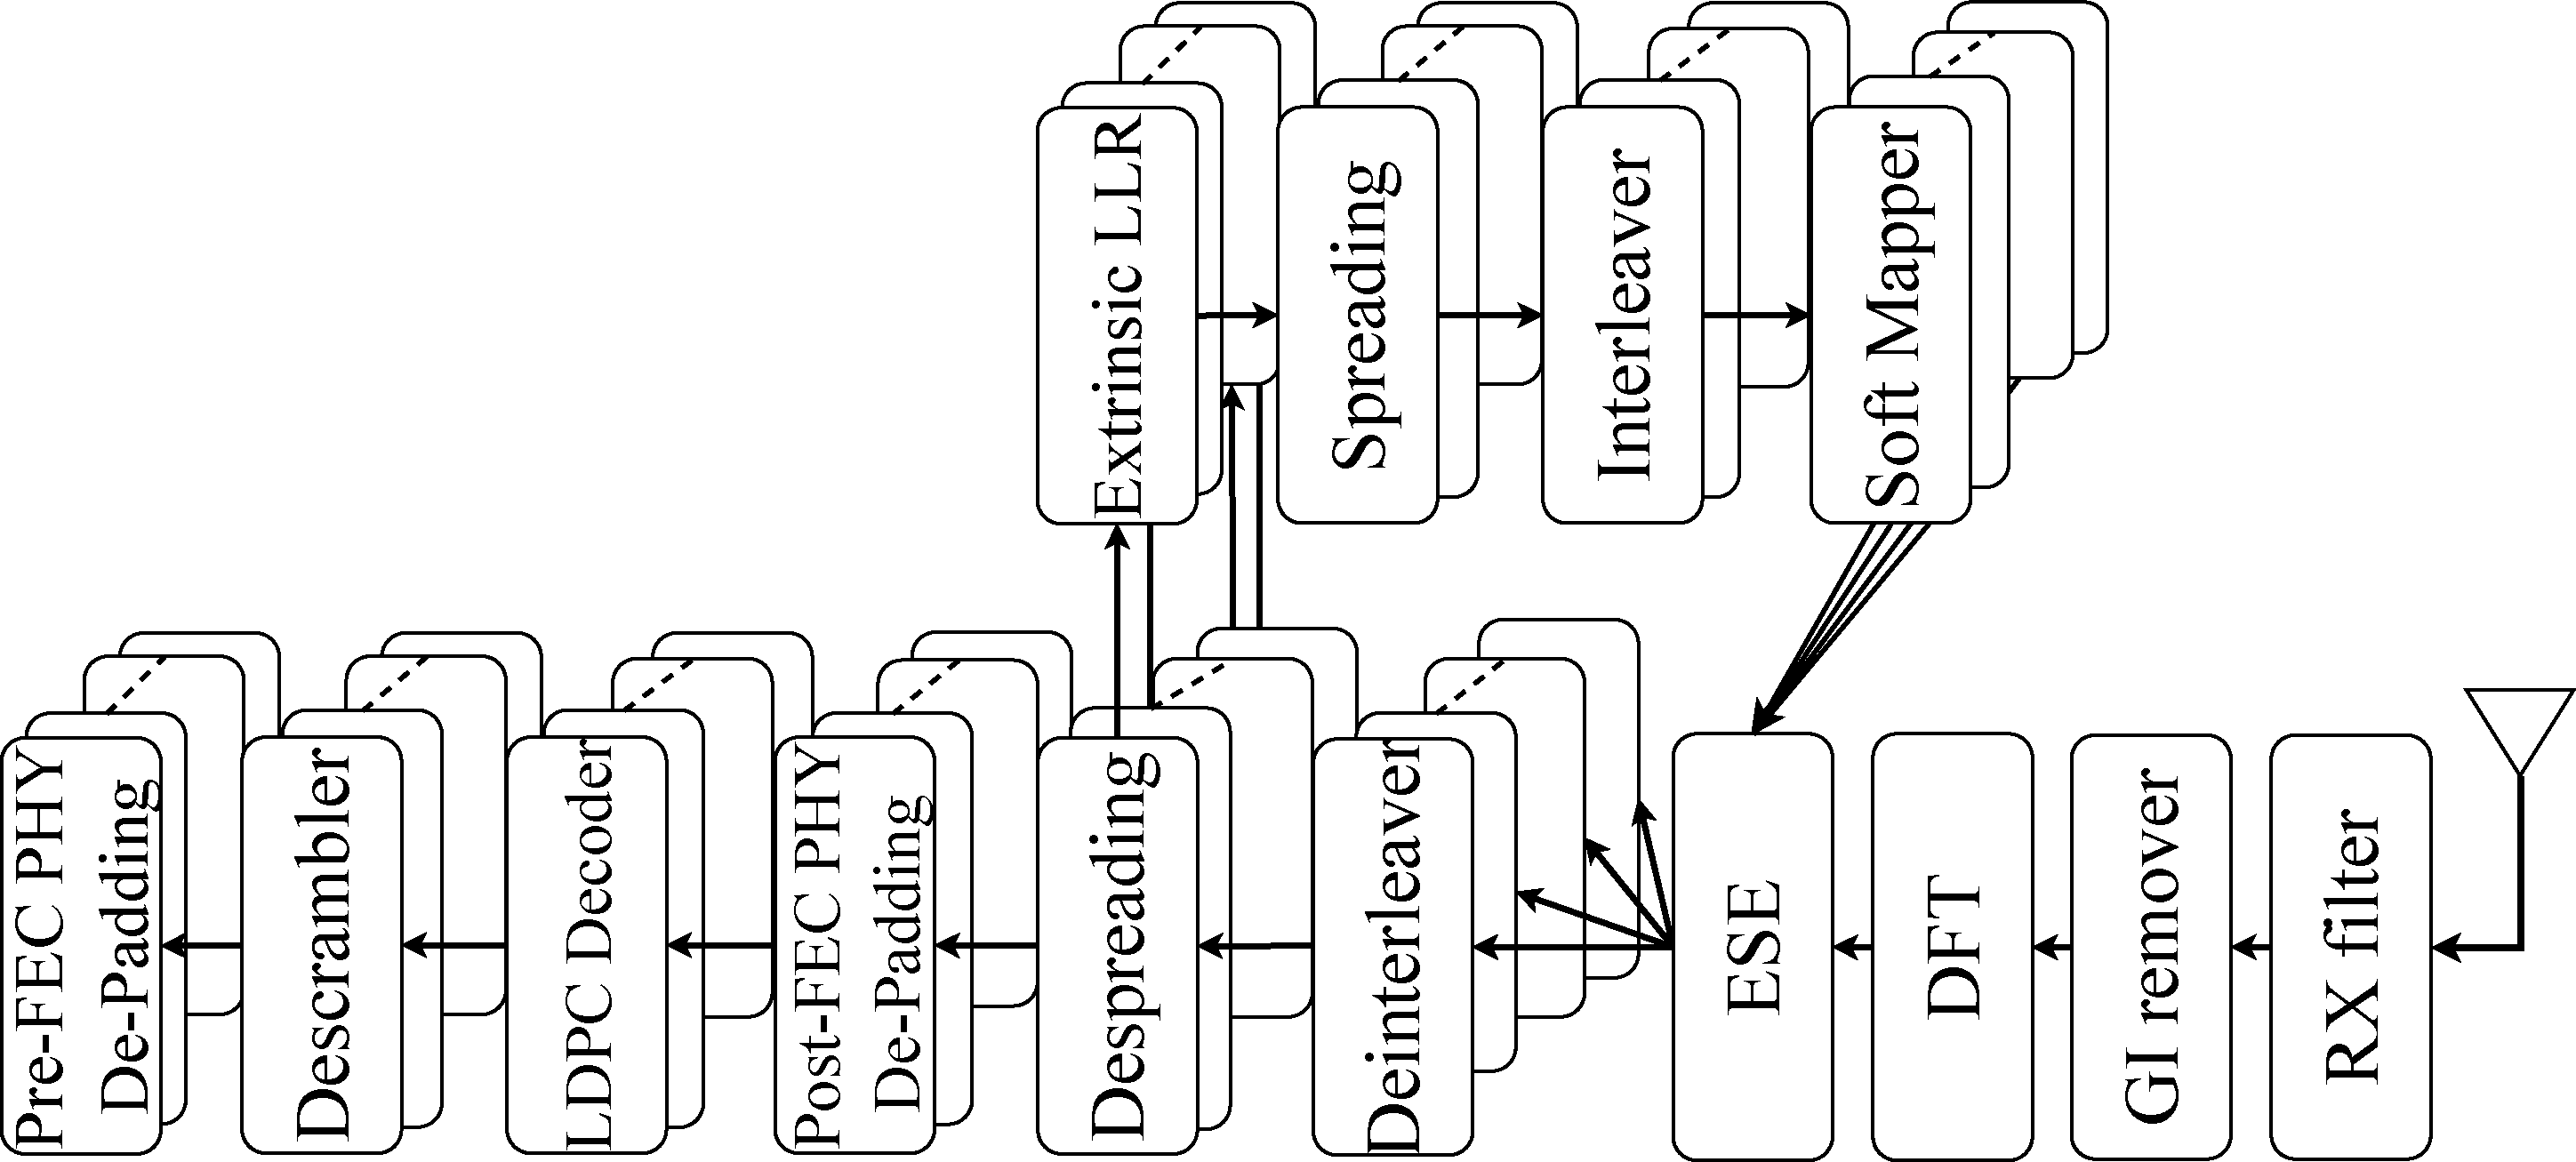
\includegraphics[width=0.75\linewidth]{figure/chap3/Proposed_Receiver.pdf}
	\caption{Proposed receiver architecture.}
	\label{fig:OFDMA-IDMARx}
	% \vspace{-1em}
\end{figure}

\chapter{KẾT QUẢ HIỆU NĂNG MÔ PHỎNG}
\label{Chap:IV}
Các kết quả của mô hình OFDMA-IDMA đề xuất được mô phỏng và đánh giá để đánh giá hiệu suất so với các kỹ thuật hiện có trong 802.11ax. Các tham số mô hình OFDMA-IDMA chi tiết được nêu trong Bảng \ref{tab:Para}. Bội số SF sẽ giảm số bit dữ liệu để điều chỉnh kích thước gói của hệ thống OFDMA-IDMA theo tiêu chuẩn 802.11.

\begin{table}[H]
	\normalsize
	\centering
	\caption{Thông số mô phỏng}
	\label{tab:Para}
	\begin{tabular}{|l|l|}
		\hline
		\textbf{Parameters}   & \textbf{Value}       \\ \hline
		Mô hình kênh          & TGax Channel Model B \\ \hline
		Băng thông            & 20 MHz               \\ \hline
		Số lượng RU chơ IDMA  & 4                    \\ \hline
		Số lượng STA          & 8, 12, 16, 20, 24    \\ \hline
		Hệ số trải (SF)       & 2                    \\ \hline
		Kiểu điều chế         & 16-QAM               \\ \hline
		Số lượng ăng-ten thu  & 4, 8                 \\ \hline
		Số vòng lặp           & 4                    \\ \hline
		Mã hóa kênh           & LDPC                 \\ \hline
		Packet length         & 1000 Bytes           \\ \hline
		Số lượng lặp mô phỏng & 1000                 \\ \hline
	\end{tabular}
\end{table}
%=====================
Hình \ref{fig:IT} cho thấy sự tác động của số lần lặp đến hiệu suất BER của OFDMA-IDMA. Khi số lần lặp tăng lên, BER được cải thiện rõ rệt. Tuy nhiên, điều cần thiết là phải xem xét sự đánh đổi với độ trễ, độ trễ có xu hướng tăng tuyến tính theo số lần lặp, để tạo sự cân bằng giữa độ trễ và chất lượng tín hiệu là rất quan trọng.
Đối với 802.11 \acrshort{OFDM} PHY, lý tưởng nhất là quá trình nhận phải được hoàn thành trong vòng 16 $\mu s$. Xem xét các yếu tố thực tế, bao gồm độ trễ xử lý đường truyền và \acrshort{MAC}, độ trễ xử lý mục tiêu nhận khoảng 10 $\mu s$ được khuyến nghị trong \cite{UL-OFDM-IDMA}.
Các tác giả này đã nghiên cứu mối quan hệ giữa số lần lặp và độ trễ trong các kịch bản OFDM-IDMA. Đối với SF bằng 2, độ trễ của hệ thống là khoảng 6 $\mu s$ cho 4 lần lặp, trong khi nó vượt quá 10 $\mu s$ cho 8 lần lặp. Do đó, báo cáo này đã chọn ra 4 lần lặp lại là một sự thỏa hiệp phù hợp để đáp ứng các yêu cầu về chất lượng và độ trễ.

\begin{figure}
	\pgfplotsset{width=0.75\linewidth,height=10cm,
		x label style={at={(axis description cs:0.5 , -0.05)},anchor=north},
		y label style={at={(axis description cs:-0.125, 0.5)},anchor=south},
		xmajorgrids,
		ymajorgrids,
	}
	\pgfplotsset{yticklabel style={text width=2em,align=right}}
	\centering
	% This file was created with tikzplotlib v0.10.1.
\begin{tikzpicture}

\definecolor{darkturquoise0191191}{RGB}{0,191,191}
\definecolor{darkviolet1910191}{RGB}{191,0,191}
\definecolor{green01270}{RGB}{0,127,0}
\definecolor{lightgray204}{RGB}{204,204,204}
\definecolor{darktangerine}{RGB}{1.0, 0.66, 0.07}

\begin{axis}[
legend cell align={left},
legend style={
  fill opacity=0.8,
  draw opacity=1,
  text opacity=1,
  at={(0.03,0.03)},
  anchor=south west,
  draw=lightgray204
},
log basis y={10},
tick pos=left,
xlabel={SNR [dB]},
xmajorgrids,
xmin=9.5, xmax=20.5,
xminorgrids,
xtick style={color=black},
ylabel={BER},
ymajorgrids,
ymin=2.16482046582444e-05, ymax=0.513035557901541,
yminorgrids,
ymode=log,
ytick style={color=black},
% ytick={1e-06,1e-05,0.0001,0.001,0.01,0.1,1,10},
% yticklabels={
%   \(\displaystyle {10^{-6}}\),
%   \(\displaystyle {10^{-5}}\),
%   \(\displaystyle {10^{-4}}\),
%   \(\displaystyle {10^{-3}}\),
%   \(\displaystyle {10^{-2}}\),
%   \(\displaystyle {10^{-1}}\),
%   \(\displaystyle {10^{0}}\),
%   \(\displaystyle {10^{1}}\)
% }
]
\addplot [semithick, blue, mark=o, mark size=3, mark options={solid}]
table {%
10 0.342706880040323
12 0.273475378024194
14 0.217120236895161
16 0.18451154233871
18 0.163001108870968
20 0.154058669354839
};
\addlegendentry{Số lần lặp = 1}
\addplot [semithick, darkviolet1910191, mark=triangle, mark size=3, mark options={solid}]
table {%
10 0.22259236391129
12 0.103527570564516
14 0.0351042842741935
16 0.0120323588709677
18 0.00708961693548387
20 0.00545539314516129
};
\addlegendentry{Số lần lặp = 2}
\addplot [semithick, darkturquoise0191191, mark=diamond, mark size=3, mark options={solid}]
table {%
10 0.196327394153226
12 0.0706490675403226
14 0.0148261340725806
16 0.00169695060483871
18 0.000602318548387097
20 0.000296421370967742
};
\addlegendentry{Số lần lặp = 4}
\addplot [semithick, green01270, mark=square, mark size=3, mark options={solid}]
table {%
10 0.194996824596774
12 0.0680136088709677
14 0.0130689516129032
16 0.00123087197580645
18 0.000225478830645161
20 0.000107258064516129
};
\addlegendentry{Số lần lặp = 8}
\addplot [ultra thick, loosely dashed, darktangerine, forget plot]
  table {%
  9.5 0.001
  20.5 0.001
  };
  \node[] at (axis cs: 12, 1.5e-3) {BER tham chiếu};
\end{axis}

\end{tikzpicture}

	\caption{Ảnh hưởng của số lần lặp với STA = 20, NRx = 8.}
	\label{fig:IT}
	% \vspace{-1em}
\end{figure}
%==========================

Hình \ref{fig:bersec4} mô tả BER trung bình cho các kỹ thuật 802.11ax sử dụng bộ cân bằng Lỗi bình phương trung bình tối thiểu (\acrshort{MMSE}) ở bộ thu với số lượng STA và ăng-ten thu (NRx) khác nhau trong băng thông 20 MHz.
Hình \ref{fig:BER MU-MIMO} thể hiện BER của kỹ thuật MU-MIMO có thể thấy được MU-MIMO rất nhạy cảm với nhiễu MAI. Ngay cả trong điều kiện tối ưu với 4 STA được truyền tới AP 8 ăng-ten, việc đạt được BER tham chiếu vẫn còn khó khăn.
Hình \ref{fig:BER OFDMA} minh họa BER của OFDMA, cho thấy ảnh hưởng MAI giảm khi STA truyền trong các RU khác nhau. Đối với 4 STA và NRx là 8, BER giảm xuống dưới $10^{-3}$ ở mức 20~[dB]. Tuy nhiên, khi số lượng STA tăng lên thì BER của OFDMA cũng tăng do nhiễu tích lũy tăng lên. Lý do là tỷ lệ giữa số điểm FFT với số lượng sóng mang trên mỗi RU sẽ tăng khi số lượng STA tăng, dẫn đến hiệu ứng tích lũy nhiễu sẽ lớn hơn khi số lượng STA tăng.
Hình \ref{fig:BER OFDMA-MU-MIMO} hiển thị BER trung bình của OFDMA-MU-MIMO với trường hợp số RU là 2, đây là kích thước RU tối thiểu để triển khai OFDMA-MU-MIMO ở 20 MHz trong 802.11ax \cite{IEEEStd}. Mặc dù OFDMA-MU-MIMO mang lại hiệu suất phổ cao hơn OFDMA khi số lượng STA tăng lên, nhưng nó phải đối mặt với những thách thức trong việc đạt được BER tham chiếu, nhưng BER của nó vẫn vượt trội hơn so với phương án sử dụng MU-MIMO.

Hình \ref{fig:BER OFDMA-IDMA} minh họa BER trung bình trong OFDMA-IDMA được đề xuất với 4 RU. Có thể thấy tốc độ dữ liệu của OFDMA-IDMA sẽ giảm đi một nửa so với các kỹ thuật khác nêu trên khi chọn SF là 2, tuy nhiên chất lượng và số lượng STA tăng lên đáng kể so với các kỹ thuật đó. Khi đặt cạnh trường hợp chia RU và nhiều STA trong một RU như được mô tả trong Hình \ref{fig:BER OFDMA-MU-MIMO}, kỹ thuật OFDMA-IDMA được đề xuất sẽ vượt trội hơn. Xem xét trường hợp tốt nhất của OFDMA-MU-MIMO với 4 STA và 8 ăng-ten thu (STA~=~4, NRx = 8), BER xấp xỉ $10^{-2}$ tại SNR~=~20 [dB]. Tuy nhiên, đối với ba kỹ thuật trong hình \subref{fig:BER MU-MIMO}, \subref{fig:BER OFDMA}, \subref{fig:BER OFDMA-MU-MIMO}, giả sử việc đánh đổi việc giảm tốc độ bằng một nửa tốc độ dữ liệu và nhân đôi số lượng STA là hợp lý, vì vậy trường hợp tốt nhất OFDMA-IDMA (STA = 8 , NRx~=~8) đạt được hầu như không có lỗi ở SNR~=~20 [dB]. Tuy nhiên, so với OFDMA thông thường, trong đó trường hợp tốt nhất (STA~=~4, NRx = 8) mang lại BER khoảng $3\mathord{\times}10^{-4}$ tại SNR~=~20 [dB] đạt được BER tham chiếu thì rõ ràng OFDMA-IDMA vẫn cho kết quả tốt hơn nhiều (STA~=~8, NRx = 8).
Ngoài ra, kỹ thuật đề xuất còn triển khai MU đường lên trong 4 RU, điều mà MU-MIMO không thể đạt được trong 802.11ax. Về mặt hiệu quả phổ tần, việc triển khai OFDMA-IDMA ở 4 RU sẽ giảm hai lần so với 2 RU như MU-MIMO, nhưng chất lượng truyền dẫn cũng như số lượng STA sẽ tăng lên đáng kể.
Sự đánh đổi này đáng được xem xét trong trường hợp OFDMA-MU-MIMO tốt nhất (STA = 4, NRx = 8); BER của kỹ thuật này vẫn chưa thể đạt tới ngưỡng tham chiếu ở mức 20 dB. Đối với OFDMA-IDMA, khi xem xét tăng số lượng STA lên 20, BER vẫn xấp xỉ $3\mathord{\times}10^{-4}$, nghĩa là mặc dù tốc độ dữ liệu hoặc hiệu suất phổ giảm đi một nửa, số lượng STA tăng gấp 5 lần so với OFDMA. Ngay cả khi xem xét trường hợp STA~=~24 và Nrx = 8, BER của OFDMA-IDMA vẫn tiếp cận mức tham chiếu, cho thấy số lượng STA tăng gấp sáu lần so với trường hợp tốt nhất của OFDMA-MU-MIMO.


\begin{figure}
	\centering
	\pgfplotsset{width=\linewidth,height=10cm,
		x label style={at={(axis description cs:0.5 , -0.1)},anchor=north},
		y label style={at={(axis description cs:-0.2, 0.5)},anchor=south},
		xmajorgrids,
		ymajorgrids,
	}
	\pgfplotsset{yticklabel style={text width=2em,align=right}}

	\begin{subfigure}[]{0.45\linewidth}
		% This file was created with tikzplotlib v0.10.1.
\begin{tikzpicture}[scale = 1]

\definecolor{darkturquoise0191191}{RGB}{0,191,191}
\definecolor{darkviolet1910191}{RGB}{191,0,191}
\definecolor{goldenrod1911910}{RGB}{191,191,0}
\definecolor{green01270}{RGB}{0,127,0}
\definecolor{lightgray204}{RGB}{204,204,204}
\definecolor{darktangerine}{RGB}{1.0, 0.66, 0.07}

\begin{axis}[
legend cell align={left},
legend columns=2,
legend style={
  fill opacity=0.8,
  draw opacity=1,
  text opacity=1,
  at={(0.01,0.15)},
  anchor=west,
  draw=lightgray204
},
log basis y={10},
tick pos=left,
xlabel={SNR [dB]},
xmajorgrids,
xmin=9.5, xmax=20.5,
xminorgrids,
xtick style={color=black},
ylabel={BER},
ymajorgrids,
ymin=9.28649163113646e-06, ymax=0.572645816836016,
yminorgrids,
ymode=log,
ytick style={color=black},
% ytick={1e-05,0.0001,0.001,0.01,0.1,1,10},
% yticklabels={
%   \(\displaystyle {10^{-5}}\),
%   \(\displaystyle {10^{-4}}\),
%   \(\displaystyle {10^{-3}}\),
%   \(\displaystyle {10^{-2}}\),
%   \(\displaystyle {10^{-1}}\),
%   \(\displaystyle {10^{0}}\),
%   \(\displaystyle {10^{1}}\)
% }
]
\addplot [semithick, dashed, blue, mark=o, mark size=3, mark options={solid}]
table {%
10 0.495759402929494
12 0.493089219215492
14 0.484774515888779
16 0.462454288728898
18 0.41964957795432
20 0.367778891509434
};
\addlegendentry{\scriptsize STA=4, NRx=4}
\addplot [semithick, blue, mark=o, mark size=3, mark options={solid}]
table {%
10 0.487141633565045
12 0.462870562313803
14 0.393067744538232
16 0.272607032025819
18 0.162863424776564
20 0.0931232311320755
};
\addlegendentry{\scriptsize STA=4, NRx=8}
% \addplot [semithick, dashed, darkviolet1910191, mark=x, mark size=3, mark options={solid}]
% table {%
% 10 0.496456926514399
% 12 0.493548336643496
% 14 0.486620456802383
% 16 0.470138257199603
% 18 0.44634957795432
% 20 0.412961146971202
% };
% \addlegendentry{\scriptsize STA=5, NRx=4}
% \addplot [semithick, darkviolet1910191, mark=x, mark size=3, mark options={solid}]
% table {%
% 10 0.48865367428004
% 12 0.469117154915591
% 14 0.409146027805362
% 16 0.310444935451837
% 18 0.206696623634558
% 20 0.13252323733863
% };
% \addlegendentry{\scriptsize STA=5, NRx=8}
\addplot [semithick, dashed, darkviolet1910191, mark=x, mark size=3, mark options={solid}]
table {%
10 0.497733594008606
12 0.496036060079444
14 0.492732187189672
16 0.485523191823899
18 0.472735807679576
20 0.457692506620324
};
\addlegendentry{\scriptsize STA=6, NRx=4}
\addplot [semithick, darkviolet1910191, mark=x, mark size=3, mark options={solid}]
table {%
10 0.493223518702416
12 0.484519157563721
14 0.454731980304535
16 0.391884082257531
18 0.314623965574313
20 0.235754613538563
};
\addlegendentry{\scriptsize STA=6, NRx=8}
% \addplot [semithick, dashed, green01270, mark=square, mark size=3, mark options={solid,rotate=180}]
% table {%
% 10 0.498135675273088
% 12 0.496128670733437
% 14 0.494529401333522
% 16 0.489265534118315
% 18 0.481894240317776
% 20 0.473643513264293
% };
% \addlegendentry{\scriptsize STA=7, NRx=4}
% \addplot [semithick, green01270, mark=square, mark size=3, mark options={solid,rotate=90}]
% table {%
% 10 0.494164757412399
% 12 0.48773221378919
% 14 0.466358118172791
% 16 0.425929475812172
% 18 0.371793587742942
% 20 0.309308678535963
% };
% \addlegendentry{\scriptsize STA=7, NRx=8}
\addplot [semithick, dashed, darkturquoise0191191, mark=triangle, mark size=3, mark options={solid}]
table {%
10 0.498238021350546
12 0.49737166397716
14 0.496360430114201
16 0.494041506330685
18 0.488708974677259
20 0.484506501365442
};
\addlegendentry{\scriptsize STA=8, NRx=4}
\addplot [semithick, darkturquoise0191191, mark=triangle, mark size=3, mark options={solid}]
table {%
10 0.495683915714995
12 0.491379499751738
14 0.481505678997021
16 0.458321577085402
18 0.419660625620655
20 0.37813781653426
};
\addlegendentry{\scriptsize STA=8, NRx=8}
\addplot [ultra thick, loosely dashed, darktangerine, forget plot]
table {%
9.5 0.001
20.5 0.001
};
\node[] at (axis cs: 13,1.5e-3) {BER tham chiếu};
\end{axis}

\end{tikzpicture}

		\vspace{-1.5em}
		\caption{BER của MU-MIMO.}\label{fig:BER MU-MIMO}
	\end{subfigure}
	\begin{subfigure}[]{0.45\linewidth}
		% This file was created with tikzplotlib v0.10.1.
\begin{tikzpicture}[scale = 1]

\definecolor{darkturquoise0191191}{RGB}{0,191,191}
\definecolor{darkviolet1910191}{RGB}{191,0,191}
\definecolor{green01270}{RGB}{0,127,0}
\definecolor{lightgray204}{RGB}{204,204,204}
\definecolor{darktangerine}{RGB}{1.0, 0.66, 0.07}

\begin{axis}[
legend cell align={left},
legend columns=2,
legend style={
  fill opacity=0.8,
  draw opacity=1,
  text opacity=1,
  at={(0.01,0.15)},
  anchor=west,
  draw=lightgray204
},
log basis y={10},
tick pos=left,
xlabel={SNR [dB]},
xmajorgrids,
xmin=9.5, xmax=20.5,
xminorgrids,
xtick style={color=black},
ylabel={BER},
ymajorgrids,
ymin=9.28649163113646e-06, ymax=0.572645816836016,
yminorgrids,
ymode=log,
ytick style={color=black},
% ytick={1e-05,0.0001,0.001,0.01,0.1,1,10},
% yticklabels={
%   \(\displaystyle {10^{-5}}\),
%   \(\displaystyle {10^{-4}}\),
%   \(\displaystyle {10^{-3}}\),
%   \(\displaystyle {10^{-2}}\),
%   \(\displaystyle {10^{-1}}\),
%   \(\displaystyle {10^{0}}\),
%   \(\displaystyle {10^{1}}\)
% }
]
\addplot [semithick, dashed, blue, mark=o, mark size=3, mark options={solid}]
table {%
10 0.38003634375
12 0.24171484375
14 0.1196720625
16 0.05172925
18 0.019391
20 0.00756159375
};
\addlegendentry{\scriptsize STA=4, NRx=4}
\addplot [semithick, blue, mark=o, mark size=3, mark options={solid}]
table {%
10 0.2608909375
12 0.1283121875
14 0.042170625
16 0.009151875
18 0.0018371875
20 0.0003165625
};
\addlegendentry{\scriptsize STA=4, NRx=8}
\addplot [semithick, dashed, darkviolet1910191, mark=x, mark size=3, mark options={solid}]
table {%
10 0.3653874185502
12 0.244531814935065
14 0.137767682239635
16 0.0694292653752498
18 0.0330769410433317
20 0.01451406685502
};
\addlegendentry{\scriptsize STA=8, NRx=4}
\addplot [semithick, darkviolet1910191, mark=x, mark size=3, mark options={solid}]
table {%
10 0.273217060876623
12 0.145498864541708
14 0.0602944973464036
16 0.0212365223682567
18 0.00610429470529471
20 0.00145596714223277
};
\addlegendentry{\scriptsize STA=8, NRx=8}
\addplot [semithick, dashed, darkturquoise0191191, mark=triangle, mark size=3, mark options={solid}]
table {%
10 0.361804513888889
12 0.241939041666667
14 0.139245861111111
16 0.0715146805555556
18 0.0355674583333333
20 0.0165399444444444
};
\addlegendentry{\scriptsize STA=9, NRx=4}
\addplot [semithick, darkturquoise0191191, mark=triangle, mark size=3, mark options={solid}]
table {%
10 0.277957
12 0.147020666666667
14 0.0593184722222222
16 0.0205094305555556
18 0.00571811111111111
20 0.00159363888888889
};
\addlegendentry{\scriptsize STA=9, NRx=8}
\addplot [ultra thick, loosely dashed, darktangerine, forget plot]
  table {%
  9.5 0.001
  20.5 0.001
  };
\node[] at (axis cs: 13, 1.5e-3) {BER tham chiếu};
\end{axis}

\end{tikzpicture}

		\vspace{-1.5em}
		\caption{BER của OFDMA.}\label{fig:BER OFDMA}
	\end{subfigure}

	\vspace{1cm}
	%================================
	\begin{subfigure}[]{0.45\linewidth}
		% This file was created with tikzplotlib v0.10.1.
\begin{tikzpicture}[scale = 1]

\definecolor{darkturquoise0191191}{RGB}{0,191,191}
\definecolor{darkviolet1910191}{RGB}{191,0,191}
\definecolor{goldenrod1911910}{RGB}{191,191,0}
\definecolor{green01270}{RGB}{0,127,0}
\definecolor{lightgray204}{RGB}{204,204,204}
\definecolor{darktangerine}{RGB}{1.0, 0.66, 0.07}

\begin{axis}[
legend cell align={left},
legend columns=2,
legend style={
  fill opacity=0.8,
  draw opacity=1,
  text opacity=1,
  at={(0.01,0.15)},
  anchor=west,
  draw=lightgray204
},
log basis y={10},
tick pos=left,
tick align=inside,
xlabel={SNR [dB]},
xmajorgrids,
xmin=9.5, xmax=20.5,
xminorgrids,
xtick style={color=black},
ylabel={BER},
ymajorgrids,
ymin=9.28649163113646e-06, ymax=0.572645816836016,
yminorgrids,
ymode=log,
ytick style={color=black},
% ytick={1e-08,1e-07,1e-06,1e-05,0.0001,0.001,0.01,0.1,1,10,100}
% yticklabels={
%   \(\displaystyle {10^{-9}}\),
%   \(\displaystyle {10^{-8}}\),
%   \(\displaystyle {10^{-7}}\),
%   \(\displaystyle {10^{-6}}\),
%   \(\displaystyle {10^{-5}}\),
%   \(\displaystyle {10^{-4}}\),
%   \(\displaystyle {10^{-3}}\),
%   \(\displaystyle {10^{-2}}\),
%   \(\displaystyle {10^{-1}}\),
%   \(\displaystyle {10^{0}}\),
%   \(\displaystyle {10^{1}}\)
% }
]
\addplot [semithick, dashed, blue, mark=o, mark size=3, mark options={solid}]
  table {%
  10 0.475414311849512
  12 0.427380552788845
  14 0.328055577689243
  16 0.216280490537849
  18 0.126077981822709
  20 0.0715704961404383
  };
  \addlegendentry{\scriptsize STA=4, NRx=4}
  \addplot [semithick, blue, mark=o, mark size=3, mark options={solid}]
  table {%
  10 0.420903230826693
  12 0.281042517430279
  14 0.152157899651394
  16 0.0647917081673307
  18 0.0242504980079681
  20 0.0092628859561753
  };
  \addlegendentry{\scriptsize STA=4, NRx=8}
  \addplot [semithick, dashed, darkviolet1910191, mark=x, mark size=3, mark options={solid}]
  table {%
  10 0.485489402805445
  12 0.458627321962151
  14 0.398791131308101
  16 0.314991239209827
  18 0.237854262118194
  20 0.174035113711819
  };
  \addlegendentry{\scriptsize STA=6, NRx=4}
  \addplot [semithick, darkviolet1910191, mark=x, mark size=3, mark options={solid}]
  table {%
  10 0.43927214060425
  12 0.327331382802125
  14 0.202177851095618
  16 0.114883507636122
  18 0.0579899983399734
  20 0.0287592338977424
  };
  \addlegendentry{\scriptsize STA=6, NRx=8}
  \addplot [semithick, dashed, darkturquoise0191191, mark=triangle, mark size=3, mark options={solid}]
  table {%
  10 0.493769644858068
  12 0.485925491782868
  14 0.465015418015438
  16 0.427567000747012
  18 0.380129934947709
  20 0.33273046875
  };
  \addlegendentry{\scriptsize STA=8, NRx=4}
  \addplot [semithick, darkturquoise0191191, mark=triangle, mark size=3, mark options={solid}]
  table {%
  10 0.478601375747012
  12 0.430529927166335
  14 0.353783771165339
  16 0.247454494521912
  18 0.167064414218127
  20 0.103025740786853
  };
  \addlegendentry{\scriptsize STA=8, NRx=8}
\addplot [ultra thick, loosely dashed, darktangerine, forget plot]
  table {%
  9.5 0.001
  20.5 0.001
  };
\node[] at (axis cs: 13, 1.5e-3) {BER tham chiếu};
\end{axis}

\end{tikzpicture}

		\vspace{-1.5em}
		\caption{BER của OFDMA-MU-MIMO.} \label{fig:BER OFDMA-MU-MIMO}
	\end{subfigure}
	\begin{subfigure}[]{0.45\linewidth}
		% This file was created with tikzplotlib v0.10.1.
\begin{tikzpicture}[scale = 1]

\definecolor{darkturquoise0191191}{RGB}{0,191,191}
\definecolor{darkviolet1910191}{RGB}{191,0,191}
\definecolor{green01270}{RGB}{0,127,0}
\definecolor{lightgray204}{RGB}{204,204,204}
\definecolor{darktangerine}{RGB}{1.0, 0.66, 0.07}
% \scriptsize
  \begin{axis}[
  legend cell align={left},
  legend columns=2,
  legend style={
    fill opacity=0.8,
    draw opacity=1,
    text opacity=1,
    at={(0.01,0.15)},
    anchor=west,
    draw=lightgray204
  },
  log basis y={10},
  tick pos=left,
  xlabel={SNR [dB]},
  xmajorgrids,
  xmin=9.5, xmax=20.5,
  xminorgrids,
  xtick style={color=black},
  ylabel={BER},
  ymajorgrids,
  % ymin=9.28649163113646e-06, ymax=0.572645816836016,
  ymin=8.28649163113646e-11, ymax=0.572645816836016,
  yminorgrids,
  ymode=log,
  ytick style={color=black},
  % ytick={1e-09,1e-08,1e-07,1e-06,1e-05,0.0001,0.001,0.01,0.1,1,10},
  % yticklabels={
  %   \(\displaystyle {10^{-9}}\),
  %   \(\displaystyle {10^{-8}}\),
  %   \(\displaystyle {10^{-7}}\),
  %   \(\displaystyle {10^{-6}}\),
  %   \(\displaystyle {10^{-5}}\),
  %   \(\displaystyle {10^{-4}}\),
  %   \(\displaystyle {10^{-3}}\),
  %   \(\displaystyle {10^{-2}}\),
  %   \(\displaystyle {10^{-1}}\),
  %   \(\displaystyle {10^{0}}\),
  %   \(\displaystyle {10^{1}}\)
  % }
  ]
  %==========STA = 8
  \addplot [semithick, dashed, blue, mark=o, mark size=3, mark options={solid}]
  table {%
  10 0.105542086693548
  12 0.03317578125
  14 0.00980342741935484
  16 0.00169695060483871  
  18 0.000301108870967742 
  20 0.00008758064516129
  };
  \addlegendentry{\scriptsize STA=8, NRx=4 }
  \addplot [semithick, blue, mark=o, mark size=3, mark options={solid}]
  table {%
  10 0.00754063760080645
  12 0.000564415322580645
  14 0.0000329851310483871
  16 3.15020161290323e-07
  18 0
  20 0
  };
  \addlegendentry{\scriptsize STA=8, NRx=8 }
  %0.00330323840725806 18
 
  %========STA = 12
  \addplot [semithick, dashed, darkviolet1910191, mark=x, mark size=3, mark options=  {solid}]
  table {%
  10 0.219595619119624
  12 0.109079238071237
  14 0.0406001554099462
  16 0.0118438760080645
  18 0.00307266465053763
  20 0.000739961357526882
  };
  \addlegendentry{\scriptsize STA=12, NRx=4}
  \addplot [semithick, darkviolet1910191, mark=x, mark size=3, mark options={solid}]
  table {%
  10 0.0355962071572581
  12 0.00509545110887097
  14 0.000770770329301075
  16 5.35458669354839e-05
  18 4.70430107526882e-06
  20 2.52016129032258e-07
  };
  \addlegendentry{\scriptsize STA=12, NRx=8}

  %========STA = 16
  \addplot [semithick, dashed, darkturquoise0191191, mark=triangle, mark size=3,  mark options={solid}]
  table {%
  10 0.332619392641129
  12 0.215368353074597
  14 0.111528698336694
  16 0.0383162802419355
  18 0.0126934538810484
  20 0.00474168346774194
  };
  \addlegendentry{\scriptsize STA=16, NRx=4}

  \addplot [semithick, darkturquoise0191191, mark=triangle, mark size=3, mark   options={solid}]
  table {%
  10 0.0984311680947581
  12 0.0256324974798387
  14 0.0031804435483871
  16 0.000301631804435484
  18 0.0000225819052419355
  20 1.89012096774194e-06
  };
  \addlegendentry{\scriptsize STA=16, NRx=8}

  %========STA = 20
  \addplot [semithick, dashed, green01270, mark=square, mark size=3, mark options=  {solid}]
  table {%
  10 0.404963205645161
  12 0.324013810483871
  14 0.212407308467742
  16 0.116323966733871
  18 0.0588404737903226
  20 0.032302091733871
  };
  \addlegendentry{\scriptsize STA=20, NRx=4}
  %0.00169695060483871 18
  \addplot [semithick, green01270, mark=square, mark size=3, mark options={solid}]
  table {%
  10 0.196327394153226
  12 0.0706490675403226
  14 0.0148261340725806
  16 0.00330323840725806  
  18 0.000602318548387097
  20 0.000296421370967742
  };
  \addlegendentry{\scriptsize STA=20, NRx=8}

  %===========STA = 24
  \addplot [semithick, dashed, red, mark=diamond, mark size=3, mark options={solid}]
  table {%
  10 0.44402194640457
  12 0.391929918514785
  14 0.31088970094086
  16 0.21369783266129
  18 0.145292023689516
  20 0.115868048555108
  };
  \addlegendentry{\scriptsize STA=24, NRx=4}

  \addplot [semithick, red, mark=diamond, mark size=3, mark options={solid}]
  table {%
  10 0.281350806451613
  12 0.13714797547043
  14 0.039058110719086
  16 0.00865893817204301
  18 0.0025793220766129
  20 0.000844648857526882
  };
  \addlegendentry{\scriptsize STA=24, NRx=8}

  
  \addplot [ultra thick, loosely dashed, darktangerine, forget plot]
  table {%
  9.5 0.001
  20.5 0.001
  };
  \node[] at (axis cs: 13,3e-4) {BER tham chiếu};
  \end{axis}
\end{tikzpicture}


		\vspace{-0.25em}
		\caption{BER của OFDMA-IDMA.} \label{fig:BER OFDMA-IDMA}
	\end{subfigure}

	\caption{Hiệu suất BER trung bình giữa các kỹ thuật.}\label{fig:bersec4}
	\vspace{1.51em}
\end{figure}
% Although the reference BER is achieved, it is clear that OFDMA-IDMA still gives much better results (STA = 8, NRx = 8). In addition, when considering increasing the number of STAs to 20, the BER is still approximately $3\mathord{\times}10^{-4}$, meaning that even though the data rate is reduced by half, the number of STAs is increased 5 times compared to OFDMA.

% Figure \ref{fig:IT} shows the effect of the number of iterations on the BER performance of the proposed OFDMA-IDMA. The rising iteration number can reach a better BER. However, the latency must increase linearly with the number of iterations. Therefore, to ensure both latency and quality, the number of iterations chosen is 4, which gives the BER below the reference BER, and the latency will be below 10 $\mu s$ mentioned in \cite{UL-OFDM-IDMA}.

% In this context, four iterations are made. This selection yields a BER below the reference threshold and ensures that the latency remains within the specified threshold of 10 $\mu s$ discussed in \cite{UL-OFDM-IDMA}.

\chapter{KẾT LUẬN VÀ HƯỚNG PHÁT TRIỂN}
\label{Chap:V}
Bài báo cáo này đã đề xuất sự kết hợp OFDMA-IDMA để tối đa hóa số lượng STA cho UL-MU.
Chúng tôi đã đánh giá hiệu suất của hệ thống OFDMA-IDMA được đề xuất dựa trên tiêu chuẩn 802.11ax trong mô phỏng. Chúng tôi đã giới thiệu một cách tiếp cận mới kết hợp OFDMA và IDMA trong truyền dẫn đa người dùng đường lên, phân tích những ưu điểm và nhược điểm của nó so với các kỹ thuật hiện có trong 802.11ax. Nghiên cứu cũng kết hợp một sự đơn giản hóa của điều chế bậc cao và sử dụng MRC để nâng cao hiệu suất BER.
Các phát hiện này chứng minh khả năng tương thích của hệ thống với tiêu chuẩn 802.11ax hiện tại, cho thấy ứng dụng tiềm năng của nó trong các công nghệ Wi-Fi trong tương lai. Điều đặc biệt đáng chú ý là OFDMA-IDMA có thể tăng đáng kể số lượng STA lên gấp 5 lần so với OFDMA và 6 lần so với OFDMA-MU-MIMO mà vẫn duy trì chất lượng.

Mặc dù BER trung bình dễ dàng dạt được mức tham chiếu, các vấn đề công bằng giữa các STA vẫn còn chưa được giải quyết khi mà BER riêng lẻ giữa các STA vẫn còn sự khác biệt lớn. Nghiên cứu trong tương lai nhằm mục đích phân tích hệ thống được đề xuất để tăng cường tính hội tụ và công bằng một cách triệt để. Các giải pháp được đề xuất bao gồm phân bổ công suất và RU tối ưu. Ngoài ra, việc khám phá các kỹ thuật tiền mã hóa sẽ tăng cường độ mạnh mẽ của STA trước khi truyền dữ liệu.

% \chapter{Công trình công bố}
% \newpage
% \nocitePub{*}

% \bibliographystylePub{plain}
% \bibliographyPub{Publication}
% \renewcommand{\refname}{Công trình công bố}

%%============================
%%======= Publications =======
%%============================
\renewcommand\bibname{Các công trình công bố}
\begin{thebibliography}{100}
	% \bibitem{Boney96} T. V. Tai, M. P. N. Tan, L. H. Nam, N. V. Ha, and T. T. T. Nguyen,, ``Convergence Evaluation of OFDMA-IDMA Combination based on IEEE 802.11ax,'' in \emph{2024 16th International Conference on Knowledge and Smart Technology (KST)}, pp. 247--252, 2024.

	\bibitem{MG} T. V. Tai, M. P. N. Tan, N. M. Tri, N. V. Ha, and T. T. T. Nguyen, ``A High Sensitivity SQI with Peak-Amplitude Difference Variance for Wearable ECG Signals'', in \emph{2023 5th International Conference on Bio-engineering for Smart Technologies (BioSMART)}, pp. 1--4, 2023.

	\bibitem{HK} M. P. N. Tan, T. V. Tai, N. M. Tri, N. V. Ha, and T. T. T. Nguyen, ``EEG-ECG Extraction for Wearable All-in-One Healthcare Device'', in \emph{2023 6th International Conference on Electrical, Electronics and System Engineering (ICEESE)}, pp. 61--65, 2023.

	\bibitem{Pan} T. V. Tai, M. P. N. Tan, D. H. Tien, \textit{et al.}, ``Signal Quality Indices based on Skewness of Peak-Peak Interval for Wearable ECG Devices'', in \emph{2023 Signal Processing: Algorithms, Architectures, Arrangements, and Applications (SPA)}, pp. 42--47, 2023.

	\bibitem{MG} T. V. Tai, M. P. N. Tan, N. M. Tri, N. V. Ha, and T. T. T. Nguyen, ``Signal Quality Indices Based on Gain of Amplitude Difference for Wearable ECG Signals'', in \emph{ 2023 International Conference on Advanced Technologies for Communications (ATC)}, pp. 19--24, 2023.

	\bibitem{MG} D. H. Tien, M. P. N. Tan, T. H. Nam, T. V. Tai, and T. T. T. Nguyen, ``A Low-Complexity R-Peak Detection Based on Exponential Weight Mean-Variance for Wearable ECG Devices'', in \emph{ 2023 International Conference on Advanced Technologies for Communications (ATC)}, pp. 415--420, 2023.
\end{thebibliography}

\renewcommand\bibname{Tài liệu tham khảo}
\bibliographystyle{IEEEtran}
\bibliography{IEEEabrv,./0-Bib/Bib_Reference}



% \nocite{*}
% \newrefsection
% \nocite{KST}
% \printbibliography[keyword={Pub}, resetnumbers = true,title=YOURNAME Publication list] 
% \bibliographystyle{IEEEtran}
% \bibliography{IEEEabrv,./0-Bib/Bib_MyPaper}

% \chapter{MINH CHỨNG SẢN PHẨM}
% \label{Chap:App}
% \input{content/Appendix}


% \Appendix{
%     \postAppendix
%     \input{content/Appendix}
% }

\end{document}